\documentclass{AIFB_ITI_Crypto_Seminar}

\usepackage{todonotes}
\usepackage{csquotes}
\usepackage{listings} 
\usepackage[backend=biber,
			sorting=none]
            {biblatex}
\usepackage{pgf-umlsd}
\usepackage{adjustbox}

%\usepackage[showframe]{geometry}

\addbibresource{Literaturdatenbank.bib}

%Seminar definieren
\Seminartitel{KASTEL-Praktikum \glqq Security\grqq}
%Semester definieren
\Semester{Wintersemester 2017/2018}
%Autor definieren
\Autor{Thomas Czogalik, Maximilian Schick}
%Matrikelnummer definieren
\Matrikelnummer{1696853, 1709879}
%Betreuer definieren
\Betreuer{Florian Patzer (IOSB), Dr. Christian Haas (IOSB)}
%Titel der Arbeit definieren
\Arbeitstitel{SMB, das (Einfalls-)Tor zur Welt}

\begin{document}
%\lstset{language=C}   
%Deckblatt und Inhaltsverzeichnis erstellen
\makeTitleAndTOC
%
% Die Seminarausarbeitung
%
\section{Motivation}
%Eingrenzung
Sobald man Datei-, Druck- und andere Serverdienste in lokalen Rechnernetzen nutzen möchte, wird ein Netzwerkprotokoll benötigt. Ein Protokoll, das dies ermöglicht, ist das Server-Message-Block-Protokoll (SMB). SMB wird in nahezu jedem privaten und firmeninternen Netz verwendet. Jedes Windows-System enthält eine Microsoft Implementierung des Protokolls. Auf Unix basierten Systemen wird der Zugriff auf Ressourcen mithilfe des freien Softwarepaket Samba ermöglicht. \par
%problem
Viele große Angriffe aus den letzten Jahren nutzten Sicherheitslücken im SMB-Protokoll aus. Einer dieser Angriffe war der Sony Picture Hack vom 24. November 2014 \cite{sony}. 
%http://www.inss.org.il/wp-content/uploads/sites/2/systemfiles/SystemFiles/No.%20646%20-%20Gabi%20and%20Dudi%20for%20web.pdf
Bei diesem veröffentlichte eine Hackergruppe vertrauliche Daten aus dem Sony Pictures Filmstudio. Zu den Daten gehörten persönliche Informationen über die Mitarbeiter, E-Mails zwischen Mitarbeitern, Informationen über die Gehälter der Führungskräfte und Kopien von damals unveröffentlichten Sony-Filmen. \par
Ein weiterer SMB bezogener Angriff ereignete sich im Mai 2017. Hierbei nutzten Hacker eine Sicherheitslücke im SMB-Protokoll, um das Schadprogramm WannaCry auf fremden Rechnern einzuschleusen \cite{wannacry}. Bei WannaCry handelt es sich um eine Ransomware, also ein Schadprogramm, das Dateien auf dem befallenen Rechner verschlüsselt und Lösegeld für die Entschlüsselung fordert. Die Malware infizierte rund 200.000 Rechner in 150 Ländern, wie in \autoref{img:wannacry_map} zu sehen ist. Darunter befanden sich auch Systeme mehrerer global tätiger Unternehmen wie Server und medizinische Ausrüstung des britischen National Health Service sowie der US-Logistikkonzern FedEx. In Deutschland war hauptsächlich die Deutsche Bahn betroffen.  \par
%\footnote{https://www.digitalhealth.net/2017/10/wannacry-impact-on-nhs-considerably-larger-than-previously-suggested/} 
%\footnote{https://www.washingtonpost.com/news/the-switch/wp/2017/06/28/fedex-delivery-unit-hit-by-worldwide-cyberattack/?utm\_term=.a1c2d0255021}
%\footnote{https://www.heise.de/newsticker/meldung/Ransomware-WannaCry-befaellt-Rechner-der-Deutschen-Bahn-3713426.html} 
%-- eternalblue, wannacry, Petya, \\
%(Mängel)
%Eigener ansatz
Mit dieser Arbeit erstellen wir einen Überblick über mehrere Angriffe und die damit einhergehenden Sicherheitslücken des SMB-Protokolls. Durch falsche Konfigurationen oder nicht aktualisierte Systeme, können Angreifer weiterhin altbekannte Sicherheitslücken ausnutzen. Dies führt dazu, dass diese Angriffe trotz ihres Alters immer noch gefährlich sein können. Dabei werden wir uns auf die Microsoft Implementierung des SMB-Protokolls beschränken, da diese am weitesten verbreitet ist. Bei der Untersuchung haben wir versucht, die folgenden Fragen zu beantworten:
\begin{itemize}
\item Zu welcher Angriffsart gehören die verschiedenen Angriffe auf das SMB-Protokoll? 
\item Wie funktionieren diese?
\item Wie sieht ein verwundbares System aus? Welche Windows Versionen sind betroffen?
\item Wie kann man sich schützen? Wie muss das System konfiguriert werden? Muss ein Patch installiert werden?
\end{itemize}
%(evaluierung)
Abschließend wird evaluiert, ob die Angriffe, die teilweise über 20 Jahre alt sind, heute noch von Bedeutung sind. Dazu wurden Testsysteme mit unterschiedlichen Betriebssystemen, in verschiedenen Versionen aufgesetzt. Mithilfe von frei verfügbaren Implementierungen der Exploits, die zum Aufzeigen einer Sicherheitslücke entwickelt wurden, soll festgestellt werden, ob beim Betreiben eines bestimmten Betriebssystems die jeweilige Sicherheitslücke ausgenutzt werden kann.\par
Die Arbeit ist wie folgt aufgebaut: In \autoref{sec:grundlagen} werden für diese Arbeit wichtige Grundlagen erläutert. \autoref{sec:angriffe} behandelt die in dieser Arbeit betrachteten Angriffe auf das SMB-Protokoll. In \autoref{sec:evaluierung} werden verschiedene Testsysteme mithilfe von Exploits angegriffen und evaluiert. Schließlich fasst \autoref{sec:zusammenfassung} die Arbeit zusammen.

\begin{figure}
\center
  \includegraphics[width=1\textwidth]{Bilder/wannacry_map.png}
  \caption{Ausbreitung von WannaCry \cite{wannacry}.}
  \label{img:wannacry_map}
\end{figure}

\section{Grundlagen}
%https://msdn.microsoft.com/en-us/library/ee441810.aspx#gt_ee1ec898-536f-41c4-9d90-b4f7d981fd67
\label{sec:grundlagen}
\subsection{Server-Message-Block (SMB)}
%- was ist SMB? 
Das SMB-Protokoll (Server-Message-Block) ist ein Netzwerkprotokoll auf Anwendungsebene. Es wird hauptsächlich für den gemeinsamen Zugriff auf Dateien, Drucker, serielle Schnittstellen und sonstige Kommunikation zwischen Knoten in einem Netzwerk verwendet. 
%- Implementierungen 
Die bekanntesten Implementierungen des Protokolls sind SAMBA~\cite{samba} und das Microsoft-SMB-Protokoll~\cite{ms_smb}. 
%-- Samba
Bei SAMBA handelt es sich um eine freie multiplattform Implementierung des SMB-Protokolls. Es wird hauptsächlich auf Unix-Systemen verwendet. 
%-- MS 
Die Microsoft Implementierung ist dagegen in allen Windows-Systemen enthalten. Im Folgenden wollen wir uns auf die Microsoft Implementierung beschränken. 
%--- Versionen
\subsubsection{Microsoft-SMB-Protokoll}
Die erste SMB-Version (SMB1) stammt aus dem Jahr 1990. SMB2 wurde 2006 mit Windows Vista eingeführt. 2012 wurde SMB3, die mittlerweile aktuellste SMB-Version, mit Windows 8 veröffentlicht. Neben SMB3 sind auch die älteren Versionen, SMB1 und SMB2, standardmäßig auf jeder aktuellen Windows Version installiert. Das mehrere Versionen parallel installiert sind, hat den Grund, dass damit auch mit Geräten kommuniziert werden kann, die ausschließlich eine ältere Version des Protokolls unterstützen. Ein Angreifer kann dies aber ausnutzen und sein Opfer dazu bringen über SMB1 mit ihm zu kommunizieren. Dadurch erhält ein Angreifer viel mehr Informationen über den Rechner, mit dem er kommunizieren will, da SMB1 über 100 Kommandos zur Kommunikation zur Verfügung stellt. 
%Ein Großteil der Angriffe auf das SMB-Protokoll nutzt somit Design- und Implementierungsfehler in SMB1 aus. 
Erst mit SMB2 wurde die Kommunikation eingeschränkt, indem aus über 100 Kommandos 19 wurden \cite{smb1_smb2}. Außerdem wurden weitere Sicherheitsmaßnahmen implementiert, um den Anwender vor verschiedenen Angriffen zu schützen. Microsoft rät deshalb dazu SMB1 nicht mehr zu verwenden und zu deinstallieren \cite{smb1_stop}. Deshalb ist seit dem Windows 10 Fall Creators Update und der Windows Server Version 1709 SMB1 nicht mehr standardmäßig installiert~\cite{fall_creator}. 
%https://blogs.technet.microsoft.com/filecab/2016/09/16/stop-using-smb1/
%https://en.wikipedia.org/wiki/Server_Message_Block#Implementation
%was sind Shares?! \\
\subsubsection{SMB-Verbindung}
Im OSI-Netzwerkmodell lässt sich das SMB-Protokoll in die Anwendungs- oder Präsentationsschicht einordnen. Zum Transport verwendet es untergeordnete Protokolle. Eine Verbindung zwischen den Kommunikationspartnern wird meist direkt über den TCP-Port 445 aufgebaut oder bei Verwendung der NetBIOS-Api über die TCP-Ports 137 und 139. Nachdem die Kommunikationspartner verbunden sind, kann nun eine SMB-Session aufgebaut werden. Dies ist in~\autoref{abb:smb_session} veranschaulicht. Zunächst müssen der Client und der Server einen SMB-Dialekt wählen~\cite{smb_dialect}. Dieser Dialekt beschreibt die höchste Funktionalität, die sowohl der Client als auch der Server unterstützen. Dies geschieht indem der Client eine Anfrage an den Server sendet, um einen Dialekt auszuhandeln (1). Dabei hängt er der Anfrage zusätzlich eine Liste mit seinen unterstützten Dialekten an. Im nächsten Schritt (2) entscheidet sich der Server für einen Dialekt und teilt diesen dem Client mit. Nun signalisiert der Client, dass er sich beim Server authentifizieren will (3). Die Authentifizierung wird in Abschnitt~\ref{auth} genauer betrachtet. Ist die Authentifizierung erfolgreich, signalisiert der Server dies dem Client und schickt ihm eine UID, mit der er ihn eindeutig identifizieren kann (4). Schlägt die Authentifizierung fehl, sendet der Server hier einen Fehlercode. Nach einer erfolgreichen Authentifizierung haben der Client und der Server eine SMB-Session aufgebaut. Jetzt kann der Client beispielsweise versuchen auf eine freigegebene Datei zuzugreifen. Zunächst muss er dem Server dazu signalisieren, dass er Zugriff auf eine bestimmte Freigabe haben will (5). Wird ihm diese gewährt erhält er eine TID (Tree ID) (6). Eine TID stellt eine offene Verbindung zu einer Freigabe dar. Eine offene TID muss innerhalb einer SMB-Verbindung eindeutig sein. Der Client kann den Server nun auffordern die Freigabe zu öffnen (7). Wenn der Client dazu berechtigt ist, sendet der Server eine ID um die Freigabe identifizieren zu können (8). Schließlich kann der Client den Server auffordern diese zu lesen (9). Der Server öffnet die Freigabe und schickt den Inhalt an den Benutzer (10).
\begin{figure}
\centering
%https://mirror.hmc.edu/ctan/graphics/pgf/contrib/pgf-umlsd/pgf-umlsd-manual.pdf
  
  \begin{sequencediagram}
    \newthread{A}{Client}{}
    \tikzstyle{inststyle}+=[below right=-0.85cm and 11cm of A]
    \newthread[gray]{B}{Server}{}
    
    \mess[1]{A}{1. SMB COM NEGOTIATE}{B}
    \mess[1]{B}{2. SMB COM NEGOTIATE}{A}
    \mess[1]{A}{3. SMB COM SESSION SETUP ANDX}{B}
    \mess[1]{B}{4. SMB COM SESSION SETUP ANDX}{A}
    \mess[1]{A}{5. SMB COM TREE CONNECT ANDX}{B}
    \mess[1]{B}{6. SMB COM TREE CONNECT ANDX}{A}
    \mess[1]{A}{7. SMB COM OPEN ANDX}{B}
    \mess[1]{B}{8. SMB COM OPEN ANDX}{A}
    \mess[1]{A}{9. SMB COM READ ANDX}{B}
    \mess[1]{B}{10. SMB COM READ ANDX}{A}
    
  \end{sequencediagram}
  \caption{\label{abb:smb_session} Darstellung einer SMB-Verbindung mit Öffnen einer Freigabe, basierend auf \cite{smb_szenario}}
\end{figure}

\clearpage
%-- TCP Aufbau
%-- Session \\
\subsubsection{SMB-Sicherheitsmodell}
%-- https://msdn.microsoft.com/en-us/library/windows/desktop/aa365234(v=vs.85).aspx\\
Das Sicherheitsmodell unterscheidet zwischen zwei Arten der Authentifizierung um auf Freigaben (Shares) zuzugreifen~\cite{smb_auth}. Eine Freigabe ist hierbei eine Datei, ein Verzeichnis oder ein Drucker.
\begin{itemize}
\item Benutzer-Authentifizierung: Damit können Systemadministratoren gezielt festlegen, welche Benutzer und Gruppen auf eine Freigabe zugreifen dürfen. Der Benutzer, der versucht auf eine Freigabe zuzugreifen, muss einen Benutzernamen und ein Kennwort angeben. Nachdem er sich authentifiziert hat, kann er auf alle Freigaben zugreifen, die für ihn freigegeben sind und nicht ebenfalls durch eine Freigabe-Authentifizierung geschützt sind. 
\item Freigabe-Authentifizierung: Im Gegensatz zur Benutzer-Authentifizierung wird hier keine Benutzeridentität festgelegt. Der Zugriff auf Freigaben wird durch ein Passwort gesteuert. Möchte man auf eine Freigabe zugreifen, muss man das jeweilige Passwort eingeben.
\end{itemize} 
%-SMB verwendet dabei eine Challenge-Response-Authentifizierungsverfahren. Hierbei sendet der Server dem Client einen zufälligen Bitfolge - die Challenge. Der Client muss nun mithilfe des notwendigen Passworts und der empfangenen Bitfolge eine Response berechnen. Dadurch kann der Client beweisen, dass er über ausreichende Anmeldeinformationen für den Zugriff verfügt.
%- NTLM
\subsubsection{NTLM}
\label{auth}
NTLM (NT LAN Manager)~\cite{ntlm} ist eines der möglichen Authentifizierungsverfahren des SMB-Protokolls. Es verwendet ein Challenge-Response-Protokoll. Im Folgenden wird eine Benutzer-Authentifizierung mithilfe von NTLM betrachtet. An dieser sind in der Regel drei Systeme beteiligt: ein Client, ein Server und ein Domänen-Controller. Hierbei möchte sich der Client beim Server authentifizieren. Der Domänen-Controller ist beteiligt, da er alle Anmeldedaten der Domäne kennt. Diese bestehen hierbei aus einem Benutzernamen und dem Passwort, des zu authentifizierenden Benutzers. Möchte sich der Client mittels eines lokalen Nutzers des Servers anmelden, kann auch der Server die Rolle des Domänen-Controllers übernehmen. Während der Authentifikation wird niemals das Passwort in Klartext durch das Netzwerk übertragen. Stattdessen muss der Client eine Berechnung durchführen, die beweist, dass er Zugriff auf die benötigten Anmeldeinformationen hat. \par 
\autoref{abb:ntlm_auth} zeigt den Ablauf einer erfolgreichen NTLM-Authentifizierung. Zunächst sendet der Client Alice dem Server Bob ihren Benutzernamen zu und signalisiert damit, dass sie sich bei ihm authentifizieren möchte. Bob generiert daraufhin eine zufällige Bitfolge und schickt sie Alice zurück. Diese Bitfolge ist die Challenge. Im Folgenden muss Alice mit Hilfe ihres Passwort-Hashes und der Challenge eine Response berechnen. Mit dieser Response muss Alice Bob beweisen, dass sie der Client ist, für den sie sich ausgibt. Für die Berechnung wird bei NTLM, je nach Version, die NTOWF\footnote{https://msdn.microsoft.com/en-us/library/cc236699.aspx} oder LMOWF\footnote{https://msdn.microsoft.com/en-us/library/cc236700.aspx} Funktion verwendet. Nachdem Alice die Response berechnet hat, schickt sie diese an Bob. 
%\todo[inline]{https://msdn.microsoft.com/en-us/library/cc236700.aspx ist der genaue Algorithmus. Ich werde da aber nicht wirklich schlau draus.} 
Nachdem Bob die Response erhalten hat, muss er die Anmeldung verifizieren. Dazu sendet er den Benutzernamen, die Challenge und die Response weiter an den Domänen-Controller. Dieser holt sich zunächst den Hash des Benutzerpassworts aus der Datenbank des Account-Managers. Im Anschluss berechnet er selbst die Response und vergleicht sein Ergebnis mit dem von Alice. Stimmen diese überein, hat Alice sich erfolgreich beim Server authentifiziert. Stimmen die Ergebnisse nicht überein, wird ihr der Zugriff verweigert.

\begin{figure}
\centering
\begin{adjustbox}{angle=90}
%https://mirror.hmc.edu/ctan/graphics/pgf/contrib/pgf-umlsd/pgf-umlsd-manual.pdf
  
  \begin{sequencediagram}
    \newthread{A}{Alice}{}
    \newinst[3.5]{B}{Bob}{}
    \newinst[3]{DC}{DomainController}{}
    \newinst[2]{AM}{AccountManager}{}
    
    \begin{call}{A}{authenticate('Alice')}{B}{challenge}
    	\begin{call}{B}{generateChallenge()}{B}{challenge}
    	\end{call}
    \end{call}
    
    \stepcounter{seqlevel}
    
    \begin{call}{A}{calculateResponse(challenge, pwHash)}{A}{response}
    \end{call}
    
    \stepcounter{seqlevel}
    
    \begin{call}{A}{respond('Alice', response)}{B}{true}
    	\begin{call}{B}{\shortstack{verify('Alice', challenge, \\response)}}{DC}{true}
        	\begin{call}{DC}{getPwHash('Alice')}{AM}{pwHash}
    		\end{call}
            
            \stepcounter{seqlevel}
            
            \begin{call}{DC}{calculateResponse(challenge, pwHash)}{DC}{comparisonResponse}
    		\end{call}
            
            \stepcounter{seqlevel}
            
            \begin{call}{DC}{equals(response, comparisonResponse)}{DC}{true}
    		\end{call}
    	\end{call}
    \end{call}
  \end{sequencediagram}
  \end{adjustbox}
  \caption{\label{abb:ntlm_auth} Darstellung eines erfolgreichen NTLM-Authentifizierungsprozesses.}
\end{figure}

\subsection{Angriffsarten}
%Klassifikation nach \cite{HANSMAN} mit jeweils Erklärung
\subsubsection{Remote-Code-Execution (RCE)}
Unter Remote-Code-Execution versteht man die Möglichkeit auf einem fremden System Programmcode auszuführen. Dadurch kann beispielsweise Schadsoftware installiert werden oder eine Backdoor eingerichtet werden. Es ist somit sogar möglich, die vollständige Kontrolle über das betroffene System zu übernehmen. Angriffe, die Remote-Code-Execution erlauben, gehören somit zur mächtigsten Angriffsart. 

Angriffe mit dieser Möglichkeit sind meistens durch Sicherheitslücken innerhalb verwendeter Programme bedingt. Somit ist es empfehlenswert, diese stets aktuell zu halten. Bei wichtigen Netzwerken, die besonderen Schutz benötigten, sollte man zusätzlich einen Überblick über bekannte Exploits, innerhalb verwendeter Programme, haben. Diese sollten anschließend getestet werden und falls Angriffe gelingen, sollten Gegenmaßnahmen getroffen werden. Hiermit kann die Wahrscheinlichkeit erhöht werden, dass diese das Netzwerk nicht beeinträchtigen können.

\subsubsection{Man-In-The-Middle (MITM)}
Ein Man-In-The-Middle-Angriff (MITM) ist ein Angriff, bei dem der Angreifer heimlich die Kommunikation zwischen Kommunikationspartnern, die glauben direkt miteinander zu kommunizieren, abfängt, weiterleitet und möglicherweise liest oder verändert~\cite{mitm}. Um sich vor einem MITM-Angriff zu schützen, hat ein Anwender wenig Spielraum, da die meisten Schutzmaßnahmen serverseitig unternommen werden müssen. \par
Eine Verteidigungsmöglichkeit, um sich vor dem Mitlesen zu schützen, ist das Verwenden einer starken Verschlüsselung zwischen den Kommunikationspartnern. Dafür muss eine gegenseitige Authentifizierung stattfinden. Im Anschluss kann ein verschlüsselter Kanal aufgebaut werden. Um sicherzugehen, dass die Kommunikation nicht manipuliert wird, können die Nachrichten von dem jeweiligen Kommunikationspartner signiert werden.

\subsubsection{Denial-Of-Service (DOS)}
Denial-Of-Service (DOS) bezeichnet die Nichtverfügbarkeit eines Dienstes, obwohl dieser verfügbar sein sollte~\cite{dos}. Häufig ist ein DOS die Folge eines Angriffs. Dabei wird die Maschine, die den Dienst anbietet, mit so vielen Verbindungsversuchen überflutet, dass sie den Dienst vorübergehend einstellt. \par
Mithilfe von strengeren Firewall Einstellungen kann das Risiko eines Angriffs reduziert werden. Dazu zählt zum Beispiel die Beschränkung der Bandbreitennutzung auf authentifizierte Benutzer. Auch Überwachungstools, die im Netzwerk nach ungewöhnlichen Aktivitäten Ausschau halten, können dabei helfen, im Falle eines Angriffs schnell reagieren zu können.

\subsection{Metasploit}
Metasploit\footnote{https://www.metasploit.com/} ist ein freies Open-Source Projekt der IT-Sicherheitsfirma Rapid7. Der Hauptbestandteil des Projekts ist das Metasploit-Framework. Dieses ist ein Werkzeug, welches Penetration-Tests ermöglicht. Es besteht aus vielen einzelnen Modulen, die erlauben, bekannte Exploits, wie in einem Baukastenprinzip, zu konfigurieren und auf ein erreichbares System anzuwenden. Für die meisten Module reicht es aus, ausschließlich Netzwerk bedingte Informationen wie IP-Adressen anzugeben. Somit ist es möglich bekannte Systeme auf Sicherheitslücken gegen bekannte Exploits zu testen. Aufgrund des Baukastenprinzips wird in den meisten Fällen kein detailliertes Wissen über die einzelnen Exploits benötigt. Bei der Evaluierung der Angriffe wird unter anderem das Metasploit-Framework verwendet.

\section{Angriffe auf SMB}
\label{sec:angriffe}
Im Folgenden sollen einige der bekanntesten SMB Angriffe genauer vorgestellt werden. Dazu wird jeweils zunächst eine Einführung über die Herkunft des Angriffs gegeben. Danach werden mögliche Angriffsszenarien beschrieben. Anschließend wird erklärt, warum der Angriff möglich ist. Abschließend werden Möglichkeiten genannt, wie man sich schützen kann.

\subsection{Pass-The-Hash}
\subsubsection{Einführung}
Bei Pass-The-Hash handelt es sich um einen Angriff auf das Challenge-Response-Authentifizierungsprotokoll NTLM von SMB. Dieser ermöglicht eine Authentifikation ohne ein dafür notwendiges Passwort in Klartext zu besitzen. Grund hierfür ist ein Designfehler innerhalb NTLM, da zur Authentifizierung das Passwort ausschließlich in gehashter Form benötigt wird. Die Theorie hinter diesem Angriff wurde erstmals 1997 von Paul Ashton veröffentlicht~\cite{pth_discuss}.

Dieser Angriff wird oft in Kombination mit dem Werkzeug PsExec\footnote{https://technet.microsoft.com/de-de/sysinternals/bb897553.aspx} verwendet. Dies ist Teil von PsTools\footnote{https://technet.microsoft.com/de-de/sysinternals/pstools.aspx}, einer Sammlung von Befehlszeilenprogramme zur Systemadministration. Nach einer vorangegangener Authentifikation ermöglicht PsExec, Programme auf einem fremden Client über SMB auszuführen. Hierfür muss im Vorfeld nichts auf dem Client installiert werden. Mit dem Passwort-Hash eines lokalen Administrators ist es möglich sich bei diesem System zu authentifizieren und Code auszuführen. Es wird also Remote-Code-Execution erreicht. Für PsExec in Kombination mit Pass-The-Hash existiert ein Metasploit-Modul\footnote{https://www.offensive-security.com/metasploit-unleashed/psexec-pass-hash/}.

\subsubsection{Angriffsszenario}
Im Folgenden soll ein mögliches Angriffsszenario zeigen, wie eine Angreifer mittels Pass-The-Hash ein gesamtes Netzwerk übernehmen kann~\cite{pth_szenario}.
\begin{enumerate}
\item Ein beliebiger Benutzer mit lokalen Administratorrechten infiziert versehentlich sein Gerät. Dies kann mittels Malware innerhalb einer Phishing-Mail passieren oder beispielsweise durch das Verwenden eines gefundenen USB-Sticks.
\item Wenn sich nun zu einem späteren Zeitpunkt ein Domänen-Administrator lokal an dem Gerät anmeldet, um beispielsweise das Gerät zu konfigurieren, kann die Malware dessen Passwort-Hash stehlen.
\item Mit dem Passwort-Hash eines Domänen-Administrators kann sich der Angreifer nun an allen Geräten in der Domäne Administratorrechte verschaffen.
\item Der Angreifer hat somit das Netzwerk übernommen.
\end{enumerate}

\subsubsection{Technische Details}
Das zuvor vorgestellte Angriffsszenario funktioniert, da nach dem lokalen Anmelden der Passwort-Hash eines Benutzers im Arbeitsspeicher des Geräts abgelegt wird. Der Grund hierfür ist das Komfortprinzip Single-Sign-On in Microsoft Windows. Dieses besagt, dass nach einem einmaligen Anmelden der Benutzer dauerhaft Zugriff auf seine Rechte hat. Um dies zu erlauben müssen für die Authentifikation notwendige Anmeldedaten zeitweise auf dem Rechner gespeichert werden. Windows ist standardmäßig so konfiguriert, dass die Daten der letzten zehn angemeldeten Benutzer aufbewahrt werden~\cite{pth}. Mithilfe lokaler Administratorrechte und bestimmter Tools ist es somit immer möglich einen Passwort-Hash herauszulesen. 

Wie in der Abbildung~\ref{abb:ntlm_auth} ersichtlich, wird an keinem Punkt innerhalb des Authentifizierungsprozesses das Passwort in Klartext benötigt. Somit kann der Hashwert direkt genutzt werden, ohne zuvor durch hohen rechnerischen Aufwand aus dem Hashwert den Klartext des Passwortes zurückzurechnen.

\subsubsection{Schutzmöglichkeiten}
Es existiert keine einfache Möglichkeit, um ein Netzwerk gezielt vor diesem Angriff zu schützen. Grundsätzlich sollte man sparsam mit den Rechten der einzelnen Benutzer umgehen und immer beachten mit welchen Rechten man sich an welchem Gerät anmeldet. Beispielsweise sollten Nutzer nur dann lokale Administratorrechte bekommen, wenn sie diese wirklich benötigen. Ebenfalls sollte sich ein Domänen-Administrator niemals lokal an einem Gerät anmelden. Es sollte stets ein Benutzer mit lokalen Administratorrechten benutzt werden, wenn Änderungen vorgenommen werden müssen~\cite{pth}. \par
Aktuelle Windows Versionen verfügen mittlerweile dennoch über Features, die Pass-The-Hash Angriffe erschweren. So verwendet Windows 10 eine Virtualisierungstechnik, den sogenannten Credential-Guard~\cite{pth_guard}, um den Zugriff auf zwischengespeicherte Hash-Werte zu blockieren. Zusätzlich verhindern spezielle Einträge in der Windows-Registrierdatenbank, dass sich ein lokaler Administrator von einem anderen System aus über SMB als Administrator authentifizieren kann~\cite{pth_schutz}.

\subsection{SMBRelay}
%http://resources.infosecinstitute.com/exploiting-windows-authentication-protocols-part-01/#gref
%http://www.xfocus.net/articles/200305/smbrelay.html
\subsubsection{Einführung}
Der SMBRelay Angriff stammt bereits aus dem Jahr 2001. Dabei handelt es sich um einen MITM-Angriff. Ziel des Angreifers ist es, sich beim Opfer (Server) als ein bereits bekannter Benutzer (Client) anzumelden. Dabei kommuniziert der Angreifer mit dem Client, als wäre er der Server und mit dem Server, als wäre er der Client. Der Angriff wurde vom Hacker \texttt{Sir Dystic} der Hacker Organisation \texttt{Cult of the Dead Cow} veröffentlicht. Ein Patch seitens Microsoft wurde erst sieben Jahre später veröffentlicht. Trotz des Patches kann die Schwachstelle, unter bestimmten Umständen, immer noch ausgenutzt werden. Mithilfe des SMBRelay-Metasploit-Moduls\footnote{https://www.rapid7.com/db/modules/exploit/windows/smb/smb\_relay} kann der Angriff, mit ein wenig Vorbereitung, reproduziert werden.


%- 21.3.2001 von 
%-- MITM: Klassisch zwischen beiden Parteien und fängt Daten ab, manipuliert und sendet diese weiter \\
%https://www.securestate.com/blog/2017/07/19/smb-relay-an-old-attack-that-just-got-way-easier
\subsubsection{Angriffsszenario}
Beim SMBRelay Angriff fügt sich der Angreifer in die Mitte der Verbindung zwischen Client und Server ein. Dies ist in \autoref{abb:ntlm_auth} veranschaulicht. Angreifer Mallory gibt sich dem Client Alice gegenüber als eigentlicher Verbindungspartner aus. Alle Anfragen von Alice an den Server Bob werden von Mallory an Bob weitergeleitet. Diesem gibt sich Mallory als Alice aus. Zu Beginn muss Mallory darauf warten, dass Alice sich bei Bob authentifizieren will. Nachdem sie die Anfrage abgefangen hat, leitet sie diese an Bob weiter und gibt sich dabei als Alice aus. Bob generiert eine Challange für Alice und schickt diese an Mallory. Mallory leitet nun die Challenge an Alice weiter, damit diese eine Response berechnet. Nachdem Alice ihre Response berechnet hat, sendet sie diese zurück an Mallory. Mallory leitet diese an Bob weiter. Bob überprüft Benutzername, Challenge und die Response, wie bereits in \autoref{abb:ntlm_auth} beschrieben. Nach erfolgreicher Überprüfung gewährt er Mallory Zugriff auf die Freigaben für Alice. Im letzten Schritt sendet Mallory eine Fehlernachricht an Alice.

\begin{figure}
\centering
\begin{adjustbox}{angle=90}
%https://mirror.hmc.edu/ctan/graphics/pgf/contrib/pgf-umlsd/pgf-umlsd-manual.pdf
  
  \begin{sequencediagram}
    \newthread{A}{Alice}{}
    %https://github.com/xuyuan/pgf-umlsd/issues/9
    \tikzstyle{inststyle}+=[below right=-0.85cm and 5cm of A]
    \newthread[gray]{M}{Mallory}{}
    \tikzstyle{inststyle}+=[below right=-0.85cm and 5cm of M]
    \newthread{B}{Bob}{}
    
    \begin{call}{A}{authenticate('Alice')}{M}{challenge}
    	\begin{call}{M}{authenticate('Alice')}{B}{challenge}
        	\begin{call}{B}{generateChallenge()}{B}{challenge}
    		\end{call}
    	\end{call}
    \end{call}
    
    \stepcounter{seqlevel}
    
    \begin{call}{A}{\shortstack{calculateResponse(challenge, \\pwHash)}}{A}{response}
    \end{call}
    
    \stepcounter{seqlevel}
    
    \begin{call}{A}{respond('Alice', response)}{M}{false}
    	\begin{call}{M}{respond('Alice', response)}{B}{true}
        	\begin{call}{B}{\shortstack{verify('Alice', challenge, \\response)*}}{B}{true}
    		\end{call}
    	\end{call}
    \end{call}
    
  \end{sequencediagram}
  \end{adjustbox}
  \caption{\label{abb:smbrelay_seq} Darstellung eines erfolgreichen SMBRelay Angriffs.}
  * siehe \autoref{abb:ntlm_auth}
\end{figure}

\clearpage
\subsubsection{Technische Details}
%https://web.archive.org/web/20090301225608/http://blog.metasploit.com/2008/11/ms08-067-metasploit-and-smb-relay.html
SMBRelay nutzt Designfehler des SMB-Protokolls aus. Konkret werden Schwächen des Authentifizierungsprotokolls NTLM ausgenutzt. Dabei leitet der Angreifer die Kommunikation über sich um und kann diese auch verändern, falls nötig. Der SMBRelay Angriff läuft auf Port 139. Das liegt daran, dass SMB vor Windows 2000 mit NetBIOS über den TCP/IP-Port 139 lief. Daher war eine NetBIOS-Sitzung erforderlich, um eine SMB-Verbindung aufzubauen. Da es sich bei Port 139 um einen privilegierten Port handelt, benötigt der Client Administratorrechte. Der Angriff funktioniert auch unter dem TCP-Port 445, der Client benötigt aber auch hier Administratorrechte. Noch dazu benötigt er Rechte um in den  Administrativen Freigabeordner \texttt{ADMIN\$} schreiben zu dürfen und um neue Windows Dienste zu erstellen und zu starten. Wenn das alles vorliegt, kann ein Angreifer, wie im zuvor dargestellten Szenario, sich als jemand anderes bei seinem Opfer anmelden. Im nächsten Schritt kann er eine ausführbare Datei erstellen, die sich wie ein Windows Dienst verhalten soll. Dieser Dienst enthält zusätzlich Shellcode, der dem Angreifer schließlich eine Shell auf dem Opfer anbieten soll. Die Datei wird zunächst im \texttt{ADMIN\$} Ordner abgelegt. Der enthaltene Dienst kann nun mithilfe des Service-Control-Managers gestartet werden. Der Shellcode wird ausgeführt, stoppt und löscht den Dienst und bietet dem Angreifer eine Shell auf dem Opfer an.

\subsubsection{Schutzmöglichkeiten}
Da der Angriff Designfehler des SMB-Protokolls ausnutzt, gibt es kein Allheilmittel. Sowohl der erste Patch aus dem Jahr 2008, als auch alle folgenden, die sich diesem Angriff widmen, lieferten nur einen kurzfristigen Schutz. Es gibt jedoch einige Möglichkeiten, um die Wahrscheinlichkeit eines Angriffes zu minimieren:
\begin{itemize}
\item Wähle ein sichereres Authentifizierungsprotokoll, zum Beispiel Keberos 
%\footnote{https://docs.microsoft.com/en-us/previous-versions/windows/it-pro/windows-server-2000/bb742516(v=technet.10)}.
\item Das NTLM-Protokoll deaktivieren. Dies schützt vor allem gegen einen Angriff mit dem SMBRelay-Metasploit-Modul.
\item Aktiviere SMB-Signing \cite{smbsigning} um sicherzugehen, dass SMB-Pakete während der Übertragung nicht manipuliert werden. Dabei wird aber die Abwärtskompatibilität eingeschränkt.
\item Da der Angriff einen Client mit Administratorrechten erfordert, sollten im Netzwerk verschiedene Domänen mit unterschiedlichen Sicherheitslevel eingerichtet werden. Jede Domäne bekommt dann nur die nötigen Rechte und die mögliche Angriffsfläche verkleinert sich dadurch.
\end{itemize}

\clearpage

\subsection{EternalBlue}
\subsubsection{Einführung}
EternalBlue ist ein Exploit, der mehrere Programmierfehler im SMB-Protokoll von Microsoft ausnutzt. Der Exploit erlaubt es dem Angreifer Schadcode auf fremden Rechner auszuführen. Er ist somit in der Lage den attackierten Rechner, sowie alle enthaltenen Daten zu kompromittieren. EternalBlue erfuhr im Mai 2017 großes mediales Interesse, als die Schwachstelle in Kombination mit dem Schadprogramm WannaCry ausgenutzt wurde. Im Common-Vulnerabilities-And-Exposures Industriestandard wird diese Schwachstelle als \texttt{CVE-2017-0144} bezeichnet~\cite{cve}. \par
Am 14. April 2017 erstellte die Hackergruppe \texttt{The Shadow Brokers} einen Blogeintrag mit dem Titel \texttt{Lost in Translation}~\cite{lostintranslation}. In diesem veröffentlichten sie das Fuzzbunch-Framework, welches angeblich von der NSA nahen Equation-Group geschrieben wurde. Dieses enthielt ausführbare Versionen von mehreren bis dahin unbekannten Exploits. Unter diesen befand sich auch ein Modul, welches EternalBlue ausnutzt, um auf anfälligen Systemen eine Hintertür einzurichten. Durch die Veröffentlichung wurde der Exploit erstmals publik. Der Aussage eines NSA Mitarbeiters zufolge benutzte der Geheimdienst die Sicherheitslücke aber schon seit mehreren Jahren~\cite{nsa}.\par
Durch Aufzeichnungen des vom EternalBlue-Modul erzeugten Datenpaketverkehr konnte das RiskSense-Cyber-Security-Research-Team die Funktionsweise nachvollziehen~\cite{eternalblue}. Mit diesem Wissen konnten sie den Exploit für das Metasploit-Framework portieren. Systemadministratoren können mit dem portierten Modul\footnote{https://www.rapid7.com/db/modules/exploit/windows/smb/ms17\_010\_eternalblue} ihre zugewiesene Systeme auf die EternalBlue Schwachstelle testen, ohne versehentlich eine Backdoor einzubauen. Das Modul ist dabei genauso wie das Vorbild aus dem Fuzzbunch-Framework nur mit Microsofts Windows XP (Server 2003) und Windows 7 (Server 2008 R2) kompatibel. Der Risikoanalyse vom RiskSense-Cyber-Security-Research-Team zufolge existiert aber auch ein nicht veröffentlichtes Modul für Windows 10. Deshalb wird im Folgenden nur die Windows 7 Implementierung betrachtet.

\subsubsection{Angriffsszenarien}
Durch EternalBlue kann ein System in jedem Netzwerk, das SMB nutzt, beliebigen Code auf jedem anderen System im Netzwerk ausführen. Durch die hohe Verbreitung von SMB gilt EternalBlue somit als ein sehr mächtiger Exploit. In Verbindung mit WannaCry wurde der Exploit genutzt, sobald ein Rechner in einem fremden lokalen Netz infiziert war. Der Schadcode konnte sich im Anschluss im Netzwerk verteilen und mehr Systeme infizieren.

\subsubsection{Technische Details}
Im Weiteren ist die Funktionsweise des Exploits für Windows 7 beschrieben. Es werden dabei zwei Parteien betrachtet. Der Angreifer und das angegriffene Windows 7 System auf dem der zum SMB-Protokoll zugehörige TCP-Port geöffnet ist. Da der Exploit aus mehreren Komponenten besteht, werden zuerst die einzelnen Bestandteile für sich behandelt. Abschließend wird erklärt wie sich die Schwachstelle daraus zusammensetzt. Die Funktionsweise ist dem Forschungsbericht von Check Point Research \cite{checkpoint} entnommen.

\paragraph{Buffer-Overflow}
\label{buffover}
Bis Windows 7 erlaubt jedes Windows System eine anonyme Authentifizierung über SMB1. Dies ist standardmäßig erlaubt, um jedem anderen Nutzer im lokalen Netz alle freigegebenen Ordner und Dateien auflisten zu können. Der authentifizierte Nutzer kann über die somit erstellte Session aber nicht direkt auf das System zugreifen. Es ist ihm aber erlaubt Datenpakete zu senden. Der Angreifer nutzt diese Möglichkeit aus, um Daten in einer nicht Windows NT kompatiblen Form zu senden. Dies ist wegen einer in das SMB-Protokoll eingebaute Umwandlung der Daten in eine kompatible Form möglich. Nach dem Empfangen der Daten werden diese, in umgewandelter Form, im Hauptspeicher abgelegt. Problem hierbei ist ein Programmierfehler innerhalb der Umwandlungsfunktion. Bei der Berechnung des benötigten Speicherplatzes für die umgewandelten Daten wird ein vom Sender kontrolliertes DWORD (4-Bytes) nur als WORD (2-Bytes) interpretiert. Dadurch werden die beiden höchstwertigen Bytes nicht beachtet, was zu einem zu kleinen Buffer für die zu schreibende Datenmenge führt. Deshalb entsteht ein Buffer-Overflow und Daten werden im angrenzenden Speicherblock überschrieben. Dies ist in \autoref{img:buffer-overflow} dargestellt.

\begin{figure}
\center
  \includegraphics[width=0.8\textwidth]{Bilder/buffer-overflow.png}
  \caption{Darstellung eines Buffer-Overflows.}
  \label{img:buffer-overflow}
\end{figure}

\paragraph{Pool-Grooming}
Zusätzlich zu der authentifizierten SMB1-Verbindung benötigt der Exploit noch mehrere SMB2-Verbindungen. Hierbei ist keine Authentifizierung nötig, da nur eine grundlegende Verbindung benötigt wird. Grund hierfür ist, dass für jede aufgebaute Verbindung ein zugehöriger Header-Block im Hauptspeicher abgelegt wird. Diese Header-Blöcke sind für den Exploit aus zwei Gründen notwendig:
\begin{itemize}
\item Erstens füllen diese Blöcke kleinere Lücken im fragmentierten Hauptspeicher auf, was zu einem zusammenhängenden Speicher führt. Es bleiben somit nur wenige größere Lücken übrig. Dies ist wichtig, da man erreichen will, dass der zuerst erwähnte Buffer-Overflow gezielt in einen von uns eingesetzten Block schreibt. Diese Technik nennt man Pool-Grooming. 
\item Zweitens enthält ein solcher Block zwei wichtige Adressen. Die eine Adresse referenziert eine Speicheradresse, an welcher alle Pakete, die über die zugehörige Verbindung empfangen werden, abgelegt werden sollen. Die andere referenziert eine Funktion, die nach Abbruch der zugehörigen Verbindung ausgeführt werden soll. Diese Funktion soll normalerweise den über die Dauer der Verbindung zugewiesenen Speicher aufräumen.
\end{itemize}

\paragraph{Hole-Connection}
Der letzte Bestandteil ist ein weiterer Programmierfehler innerhalb des Authentifizierungsprozesses in SMB1. Ein Angreifer kann eine zur Authentifizierung notwendige Anfrage so beantworten, dass im Hauptspeicher des Angegriffenen ein Speicherblock reserviert wird, über dessen exakte Größe der Angreifer Kontrolle hat. Durch Abbruch der Verbindung kann im Anschluss eine Lücke im Hauptspeicher erzeugt werden. Diese Verbindung wird deswegen als Hole-Connection bezeichnet.

\paragraph{Exploit}
Um aus diesen Komponenten einen zuverlässigen Exploit zu erstellen, werden spezielle Kenntnisse über undokumentierte Kernel-Strukturen und Implementierungsdetails innerhalb des SMB-Protokolls vorausgesetzt. Als erstes werden mehrere SMB2-Verbindungen aufgebaut. Dies führt dazu, dass viele kleinere Lücke im Hauptspeicher des angegriffenen Systems aufgefüllt werden und nur noch wenige größere Lücken übrig bleiben. In eine dieser Lücken wird anschließend ein Speicherblock durch die Hole-Connection abgelegt. Als nächster Schritt wird erneut Pool-Grooming ausgeführt. Dabei besteht eine hohe Wahrscheinlichkeit, dass einer der erzeugten Headerblöcke direkt hinter dem Speicherblock der Hole-Connection abgelegt wird. Nun wird die Hole-Connection abgebrochen. Dies führt, bei richtiger Anordnung, zu einer Speicherlücke mit festgelegter Größe vor einem Headerblock. Jetzt können, über eine anonym authentifizierte SMB1-Verbindung, Daten in einer nicht unterstützten Form, gesendet werden. Hierbei ist es wahrscheinlich, dass der umgewandelte Datenblock in die davor erzeugte Lücke abgelegt wird. Die Daten sind dabei so präpariert, dass der folgende Buffer-Overflow gezielt die zwei wichtigen Adressen im angrenzenden Header überschreibt. Überschreibt der Buffer-Overflow einen vom Angreifer nicht vorgesehenen Speicherblock, kann es zu nicht vorhersehbaren Verhalten, wie ein Bluescreen, führen. Die beiden Adressen im Header werden mit einer Adresse aus einem statischen Bereich, der Ausführung erlaubt, überschrieben. Anschließend wird über alle SMB2-Verbindungen Shellcode gesendet. Bei der Verbindung, dessen Header manipuliert wurde, landet der Shellcode direkt in einem ausführbaren Bereich. Der Abbruch aller SMB2-Verbindungen führt dadurch direkt zu einer Remote-Code-Execution. Damit kann beispielsweise eine Backdoor eingebaut werden. Diese Funktionsweise ist in \autoref{img:eternalblue_exploit} dargestellt

\clearpage

\begin{figure}
\center
  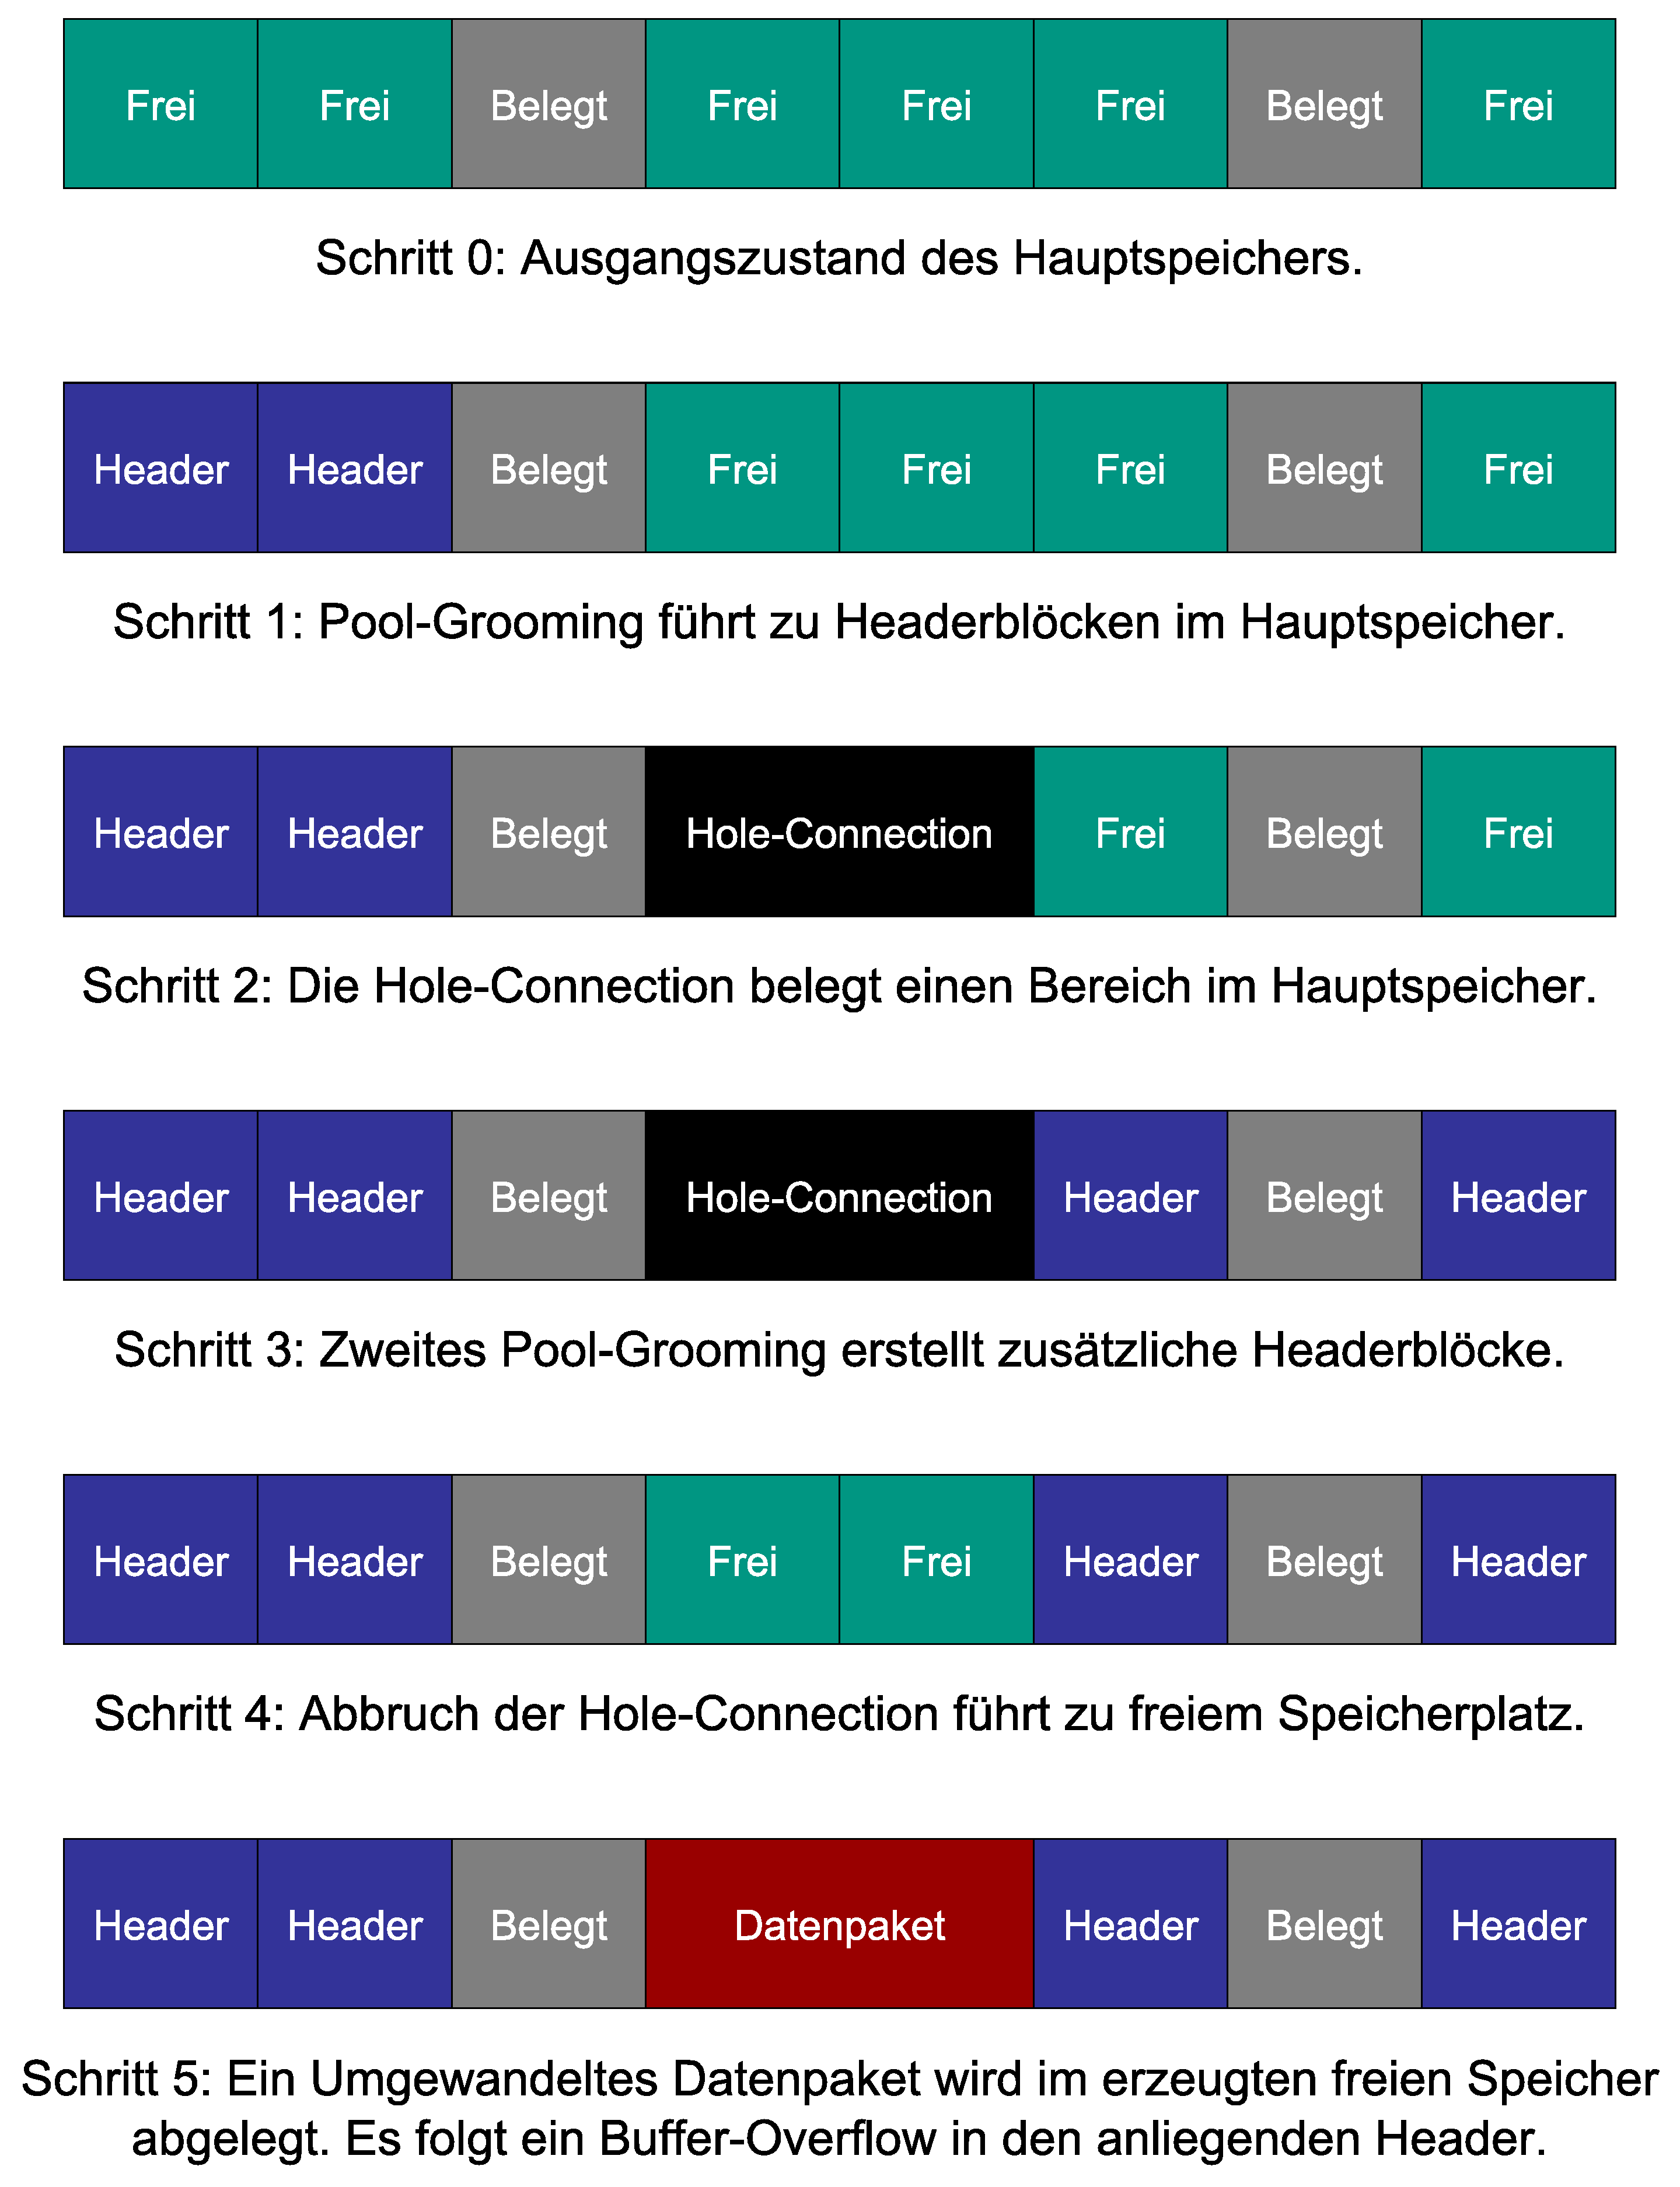
\includegraphics[width=\textwidth]{Bilder/Exploit.pdf}
  \caption{Schrittweise Darstellung des EternalBlue-Exploits.}
  \label{img:eternalblue_exploit}
\end{figure}

\clearpage

\subsubsection{Schutzmöglichkeiten}
Genau einen Monat vor der Veröffentlichung des Fuzzbunch Frameworks erschien der \texttt{MS17-010}-Patch von Microsoft~\cite{patch}. Dieser verhindert auf allen gängigen Windows Versionen den EternalBlue-Exploit. Aufgrund der schwere der Sicherheitslücke, veröffentlichte Microsoft den Patch auch für nicht mehr unterstütze Windows Versionen wie Windows XP~\cite{xp}. Der Patch beseitigt dabei nicht den zugrunde liegenden Programmierfehler, sondern fügt zusätzliche Authorisierungsabfragen beim Übermitteln von Daten ein. Es ist somit über das Netzwerk ermittelbar, ob auf einem System dieser Patch installiert ist. Hierfür gibt es Scanner im Metasploit-Framework\footnote{https://www.rapid7.com/db/modules/auxiliary/scanner/smb/smb\_ms17\_010}, in Python\footnote{https://github.com/nixawk/labs/blob/master/MS17\_010/smb\_exploit.py} und für NMAP\footnote{https://nmap.org/nsedoc/scripts/smb-vuln-ms17-010.html}. Eine weitere Möglichkeit, um sich vor dem Exploit zu schützen, ist das Deaktivieren von SMB1. Dies verhindert alle für den Exploit nötigen Schritte über dieses Protokoll. Microsoft hat bereits selbst die Gefahren, die durch das alte Protokoll ausgehen, erkannt und es mit dem Windows 10 Fall Creators Update standardmäßig auf Windows 10 deaktiviert~\cite{fall_creator}.

\subsection{SMBLoris}
\label{sub:loris}
\subsubsection{Einführung}
Dieser Angriff wurde während der Analyse von EternalBlue entdeckt. Dabei handelt es sich um einen DOS-Angriff, d.h. im Gegensatz zu den vorherigen Angriffen gibt es hier keine Codeausführung. Der SMBLoris Angriff verhält sich ähnlich zum SlowLoris Angriff \cite{banks}, weshalb er auch dessen Name geerbt hat. Beim SlowLoris öffnet eine einzelne Maschine mehrere HTTP-Verbindungen zu einem Server und hält diese so lang wie möglich offen. Andere Verbindungen können während dieser Zeit nicht verarbeitet werden. Die Besonderheit dabei ist, dass der Server nicht abstürzt, lediglich der HTTP-Server ist von dem Angriff betroffen. Von SMBLoris sind alle Windows Versionen betroffen. Auch hier ermöglicht ein Designfehler, im SMB-Protokoll, den Angriff. Dieser Fehler bezieht sich auf die Speicherallokierung beim Verbindungsaufbau einer SMB-Verbindung.

\subsubsection{Angriffsszenario}
Obwohl SMBLoris keine Code-Ausführung erlaubt, gibt es dennoch einige Szenarien in denen der Angriff Schaden anrichten kann. Da die Speicherallokierung vor dem Authentifizierungsprozess stattfindet, kann ein Angreifer beliebig viele Verbindungen zum Opfer aufmachen. In \autoref{abb:loris} ist dies veranschaulicht. Dadurch, dass der Angreifer die Verbindung halboffen lässt, wird das Opfer so sehr ausgelastet, dass es aufhört zu funktionieren. Der Angriff eignet sich beispielsweise dazu andere zu erpressen und diese so lange anzugreifen, bis diese der Forderung nachkommen. Außerdem kann der Angriff auch genutzt werden, um für Ablenkung zu sorgen. Während alle sich um den SMBLoris Angriff kümmern, können andere Angriffe ausgeführt werden, mit der Hoffnung unentdeckt zu bleiben.
\begin{figure}
\centering
\begin{sequencediagram}
	\newthread [gray]{a}{Mallory}
	\newthread {b}{Alice}
	\mess[1]{a}{SYN}{b}
    \mess[1]{a}{SYN}{b}
    \mess[1]{a}{SYN}{b}
    \stepcounter{seqlevel}
    \mess[1]{a}{...*}{b}
	
\end {sequencediagram}
  \caption{\label{abb:loris} Darstellung von mehreren halboffenen SMB-Verbindungen.}
  * insgesamt 65,535 Verbindungen
\end{figure}

\subsubsection{Technische Details}
SMBLoris nutzt einen Designfehler im SMB-Protokoll aus, der in der Speicherallokierung liegt. Der Angriff nutzt dabei den SMB-Port 445. Dabei wird beim Starten einer SMB Session zunächst der NetBIOS-Session-Service (NBSS) Header über TCP übermittelt. Dies geschieht noch bevor irgendeine Authentifikation stattgefunden hat. Der Header ist in \autoref{img:loris_header} zu sehen. Dieser benötigt 4 Bytes im Speicher des Angreifers. Das Opfer hingegen allokiert beim Empfang die angeforderte Länge von 128 KiB (2\textsuperscript{17} = 131.072-Bytes = 128 KiB). Dieser Speicher wird in einem non-paged-pool angelegt, d.h. die Daten können nicht ausgelagert werden. Das führt dazu, dass der Speicher und die CPU die gesamte Verbindung über in Anspruch genommen werden und schließlich das System zum Absturz bringen. Der Angriff nutzt dabei die Eigenschaft, dass das Öffnen einer Verbindung günstiger ist, als diese zu halten. \autoref{tab:loris_mem} zeigt die Auswirkungen auf den Speicher während des Angriffs. Dabei werden die Anzahl an aufgebauten Verbindungen skaliert. Die Tabelle zeigt zunächst, dass mit einer IP 65,535 Verbindungen aufgebaut werden können. Die Anzahl der Verbindungen ist dabei durch den TCP-Port limitiert. Dieser erlaubt 65,535 (2\textsuperscript{16}) Verbindungen. Bei dieser Anzahl an Verbindungen verbraucht der Angreifer lediglich 256 KiB an Speicher. Beim Opfer werden dagegen 8 GiB Speicher fällig. Bereits mit nur zehn IPs kann ein Angreifer mit nur 2,5 MiB Speicherverbrauch 80 GiB Speicher beim Opfer allokieren und ein Windows System somit in die Knie zwingen.
\begin{figure}
  \centering  
  \begin{tabular}{c}
  \begin{lstlisting}
  struct NBSS_HEADER
  {
      char  MessageType  : 8;
      char  Flags        : 7;
      int   Length       : 17;
  };
  \end{lstlisting}
  \end{tabular}
  \caption{Der NBSS Header \cite{loris}}
  \label{img:loris_header}
\end{figure} 

\begin{table}
\centering
\begin{tabular}{|l|c|c|c|}
\hline
Szenario & Verbindungen & Speicher (Angreifer) & Speicher (Opfer)  \\ \hline
Ausgangswert & 1 & 4 bytes & 128 KiB \\ \hline
Eine IPv4 & 65,535 & 256 KiB & 8 GiB \\ \hline
Eine IPv6 & 65,535 & 256 KiB & 8 GiB \\ \hline
Zwei IPv4/IPv6 & 131,070 & 512 KiB & 16 GiB \\ \hline
10 IPs & 655,535 & 2,5 MiB & 80 GiB \\ \hline
\end{tabular}
\caption{\label{tab:loris_mem} Speicher Allokationen während des Angriffs \cite{loris}}
\end{table}

\subsubsection{Schutzmöglichkeiten}
Obwohl alle Windows Systeme angreifbar sind plant Microsoft keinen Patch, da man grundsätzlich den ganzen Speicherallokierungsprozess ändern müsste, der seit über 20 Jahren in Betrieb ist \cite{smbpatch}. Außerdem sieht Microsoft in diesem Angriff keinen Sicherheitsfehler \cite{smbrefuse}, auch wenn es durchaus Angriffszenarien gibt. Auch Linux Systeme sind in ihrer Standardkonfiguration verwundbar. Um sich vor dem Angriff zu schützen, setzt man die maximale Anzahl der SMB-Verbindungen herunter, zum Beispiel auf 1000. Diese Konfiguration befindet sich i.d.R. in \texttt{/etc/samba/smb.conf}. Indem \texttt{max smbd processes = 1000} gesetzt wird, schützt man sich gegen den SMBLoris Angriff.

\section{Evaluierung}
\label{sec:evaluierung}
Dieser Abschnitt soll zeigen, ob und wie relevant die in \autoref{sec:angriffe} beschriebenen Angriffe heute noch sind. Dazu wurde ein Angreifersystem mit Kali Linux (Version 2017.3) aufgesetzt. Das Linux Image hierfür stammt von Offensive Security\footnote{https://www.offensive-security.com/kali-linux-vm-vmware-virtualbox-hyperv-image-download/}, einer Penetration-Testing-Website und ist bereits mit einigen Angriffswerkzeugen ausgestattet. Eins davon ist das Metasploit-Framework, mit dem die meisten unsere Angriffe durchgeführt wurden. Insgesamt gab es vier verschiedene Zielsysteme. Ein Windows 7 Professional mit Service Pack 1 (SP1), ein Windows 7 Professional mit SP1 und neuesten Updates, ein aktuelles Windows 10 mit ebenfalls allen Updates und ein Beckhoff Embedded-PC mit Windows 7 Embedded. Alle Systeme wurden mit den in \autoref{sec:angriffe} beschriebenen Angriffen attackiert. Für die Angriffe Pass-The-Hash in Kombination mit PsExec, SMBRelay und EternalBlue wurde das jeweilige Metasploit-Modul verwendet. Für Pass-The-Hash wurde dazu das standardmäßig enthaltene \texttt{RID 500} Administratorenkonto aktiviert und dessen, mittels eines Hashdump\footnote{https://www.offensive-security.com/metasploit-unleashed/meterpreter-basics/} ausgelesener, Passwort-Hash verwendet. Bei SMB-Loris wurde auf eine C-Implementierung\footnote{https://gist.github.com/marcan/6a2d14b0e3eaa5de1795a763fb58641e} zurückgegriffen. Die Ergebnisse sind in \autoref{tab:angriffs_ubersicht} zusammengefasst. Dort ist zu sehen, dass die Windows 7 Maschine ohne aktuelle Updates und trotz SP1 für alle Angriffe anfällig war. Anders sah es bei dem aktualisierten Windows 7 mit SP1 aus. Durch die Updates wurde der EternalBlue-Exploit verhindert. Außerdem wurde NTLM durch eine neuere Version ersetzt, wodurch SMBRelay nicht mehr funktionierte. Die Windows 10 Maschine war, ohne weitere Konfigurationen, gegen beiden Angriffe immun. Pass-The-Hash mittels PsExec funktionierte auf beiden neueren Versionen weiterhin. Beim Embedded-System konnten nur EternalBlue und SMBLoris untersucht werden. Für Pass-The-Hash fehlte der Passwort-Hash und für SMBRelay die Möglichkeit eine Authentifikation abzufangen und weiterzuleiten. Das System war ohne Veränderung von uns unempfindlich. SMBLoris war der einzige Angriff, der auf jeder Maschine erfolgreich war. Dieser funktionierte sowohl auf dem alten Windows 7, dem aktuellsten Windows 7, Windows 10 und Windows 7 Embedded. Die Gründe dafür wurden bereits in \autoref{sub:loris} erläutert. \par
Vor allem bei den Windows 7 Versionen wird sichtbar, dass ein aktuelles System, mit richtiger Konfiguration, vor Angriffen schützt. Für die Angriffe aus dem Metasploit-Frameworks ist nicht auszuschließen, dass diese mit anderen Implementierungen, auch auf neueren Systemen funktionieren.
\begin{table}
\centering
\begin{tabular}{|l|c|c|c|c|}
\hline
Betriebssystem & PSExec & SMBRelay & EternalBlue & SMBLoris  \\ \hline
Windows 7 Professional SP1& X & X & X & X\\ \hline
Windows 7 Professional SP1 * & X & &  & X\\ \hline
Windows 10 ** & X &  &  & X \\ \hline
Beckhoff Embedded-PC & - & - &  & X \\ \hline
\end{tabular}
\caption{\label{tab:angriffs_ubersicht} Übersicht darüber, welches System für welchen Angriff anfällig ist.}
* Inklusive Update KB4054518\footnote{https://support.microsoft.com/de-de/help/4054518}  \\
** Inklusive Update KB4053580\footnote{https://support.microsoft.com/de-de/help/4053580} 
\end{table}
\section{Zusammenfassung und Ausblick}
\label{sec:zusammenfassung}
%Zusammenfassung
In dieser Arbeit haben wir zunächst das SMB-Protokoll vorgestellt. Ein Netzwerkprotokoll, das verwendet wird, um Zugriff auf Freigaben in einem Netzwerk zu erhalten. Für dieses Protokoll haben wir vier Angriffe vorgestellt, die Design- oder Implementierungsfehler der zugehörigen Microsoft Implementierung ausnutzen. Schließlich haben wir die jeweiligen Angriffe auf Testsystemen ausgeführt, um zu prüfen, wie relevant diese heute noch sind. Das Fazit war, dass nicht aktualisierte oder falsch konfigurierte Systeme immer noch anfällig sein können. Deshalb ist es wichtig sein Netzwerk richtig abzusichern. Mögliche Sicherheitsmaßnahmen wurden bei den jeweiligen Angriffen besprochen.\par
%Adressaten der Verbesserungen
%Future Work 
Obwohl die Evaluierung gezeigt hat, dass richtig konfigurierte oder aktualisierte Systeme nicht mehr für die jeweiligen Exploits anfällig sind, schließt das andere Implementierungen der Angriffe nicht aus. Neben den verwendeten Metasploit-Modulen gibt es noch weitere Implementierungen der Angriffe, wie zum Beispiel \texttt{SMBRELAYX}\footnote{https://github.com/CoreSecurity/impacket/blob/master/examples/smbrelayx.py}. Dabei handelt es sich um eine SMBRelay Implementierung in Python, die auch mit der aktuellen NTLM Version funktioniert. Zukünftige Arbeiten könnten weitere Implementierungen der Angriffe untersuchen und prüfen, ob auch neuere Windows Versionen angreifbar sind. Außerdem wurde in dieser Arbeit nur das Microsoft-SMB-Protokoll untersucht. Weitere Arbeiten könnten die freie multiplattform Implementierung SAMBA fokussieren und untersuchen, ob und unter welchen Umständen SAMBA angreifbar ist. 
%
% Abbildungsverzeichnis
%
\clearpage
\listoffigures
%
% BibTeX Literaturverzeichnis
%
\clearpage
\printbibliography
	
\end{document}